
        \begin{tabular}{ll}
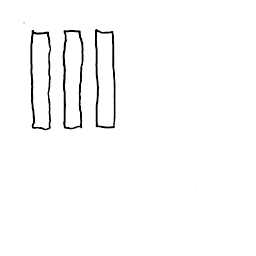
\includegraphics[width = 5cm]{../TikZ/drawings/expert-41.png}&
        \begin{minipage}{10cm}
        \begin{verbatim}
  Rectangle(2,0,3,6)
  Rectangle(4,0,5,6)
  Rectangle(0,0,1,6)
  Rectangle(0 * None + None,0,5,6)
        \end{verbatim}
\end{minipage}
\end{tabular}        
        \\

        \begin{tabular}{ll}
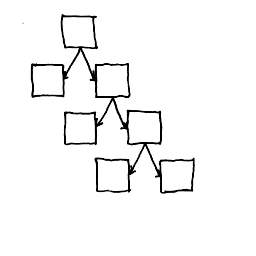
\includegraphics[width = 5cm]{../TikZ/drawings/expert-17.png}&
        \begin{minipage}{10cm}
        \begin{verbatim}
  for (4)
      Line(-2 * i + 9,3 * i + None,-2 * i + 10,3 * i + -2,arrow = True,solid = True)
      Line(-2 * i + 9,3 * i + None,-2 * i + 8,3 * i + -2,arrow = True,solid = True)
      Rectangle(2 * i + -2,-3 * i + 9,2 * i + None,-3 * i + 11)
      Rectangle(2 * i + 2,-3 * i + 9,2 * i + 4,-3 * i + 11)
        \end{verbatim}
\end{minipage}
\end{tabular}        
        \\

        \begin{tabular}{ll}

\includegraphics[width = 5cm]{../TikZ/drawings/expert-43.png}&
        \begin{minipage}{10cm}
        \begin{verbatim}
  Line(4,0,4,5,arrow = False,solid = True)
  Line(0,0,0,5,arrow = False,solid = True)
  Line(0 * None + None,0,4,5,arrow = False,solid = True)
        \end{verbatim}
\end{minipage}
\end{tabular}        
        \\

        \begin{tabular}{ll}
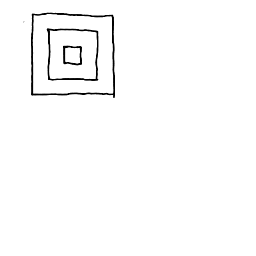
\includegraphics[width = 5cm]{../TikZ/drawings/expert-63.png}&
        \begin{minipage}{10cm}
        \begin{verbatim}
  Rectangle(2,2,3,3)
  Rectangle(1,1,4,4)
  Rectangle(0,0,5,5)
  Rectangle(1 * None + None,2,3,3)
        \end{verbatim}
\end{minipage}
\end{tabular}        
        \\

        \begin{tabular}{ll}

\includegraphics[width = 5cm]{../TikZ/drawings/expert-11.png}&
        \begin{minipage}{10cm}
        \begin{verbatim}
  Circle(1,1)
        \end{verbatim}
\end{minipage}
\end{tabular}        
        \\

        \begin{tabular}{ll}
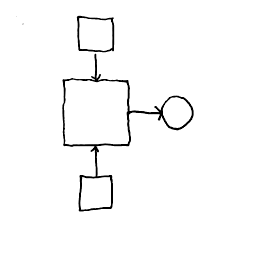
\includegraphics[width = 5cm]{../TikZ/drawings/expert-45.png}&
        \begin{minipage}{10cm}
        \begin{verbatim}
  Line(4,6,6,6,arrow = True,solid = True)
        reflect(y = 12)
        Circle(7,6)
        Line(2,2,2,4,arrow = True,solid = True)
        Rectangle(1,10,3,12)
        Rectangle(0,4,4,8)
        \end{verbatim}
\end{minipage}
\end{tabular}        
        \\

        \begin{tabular}{ll}
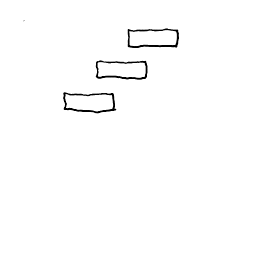
\includegraphics[width = 5cm]{../TikZ/drawings/expert-51.png}&
        \begin{minipage}{10cm}
        \begin{verbatim}
  Rectangle(0,0,3,1)
  Rectangle(2,2,5,3)
  Rectangle(4,4,7,5)
  Rectangle(4 * None + None,0,3,1)
        \end{verbatim}
\end{minipage}
\end{tabular}        
        \\

        \begin{tabular}{ll}
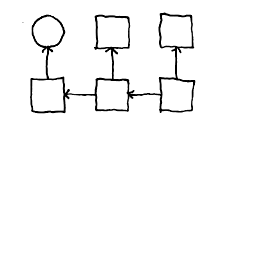
\includegraphics[width = 5cm]{../TikZ/drawings/expert-21.png}&
        \begin{minipage}{10cm}
        \begin{verbatim}
  Circle(1,5)
  Rectangle(4,4,6,6)
  Rectangle(8,4,10,6)
    for (4)
        Line(4 * i + -4,1,4 * i + -6,1,arrow = True,solid = True)
        Line(4 * i + -3,2,4 * i + -3,4,arrow = True,solid = True)
        Rectangle(4 * i + -4,0,4 * i + -2,2)
        \end{verbatim}
\end{minipage}
\end{tabular}        
        \\

        \begin{tabular}{ll}
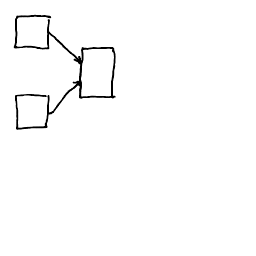
\includegraphics[width = 5cm]{../TikZ/drawings/expert-2.png}&
        \begin{minipage}{10cm}
        \begin{verbatim}
  Rectangle(4,2,6,5)
        reflect(y = 7)
        Line(2,6,4,4,arrow = True,solid = True)
        Rectangle(0,0,2,2)
        \end{verbatim}
\end{minipage}
\end{tabular}        
        \\

        \begin{tabular}{ll}
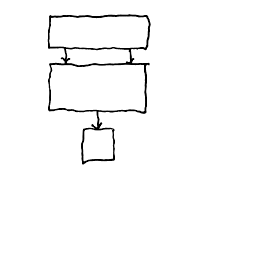
\includegraphics[width = 5cm]{../TikZ/drawings/expert-24.png}&
        \begin{minipage}{10cm}
        \begin{verbatim}
  Rectangle(0,3,6,6)
  Rectangle(2,0,4,2)
  Rectangle(0,7,6,9)
        Line(1,7,1,6,arrow = True,solid = True)
        Line(3,3,3,2,arrow = True,solid = True)
        \end{verbatim}
\end{minipage}
\end{tabular}        
        \\

        \begin{tabular}{ll}
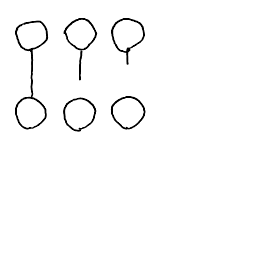
\includegraphics[width = 5cm]{../TikZ/drawings/expert-7.png}&
        \begin{minipage}{10cm}
        \begin{verbatim}
  for (3)
      Circle(3 * i + 1,6)
      Circle(-3 * i + 7,1)
      Line(3 * i + 1,None * i + 2,3 * i + 1,5,arrow = False,solid = True)
        \end{verbatim}
\end{minipage}
\end{tabular}        
        \\

        \begin{tabular}{ll}
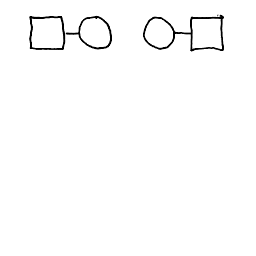
\includegraphics[width = 5cm]{../TikZ/drawings/expert-44.png}&
        \begin{minipage}{10cm}
        \begin{verbatim}
      reflect(x = 12)
      Circle(8,1)
      Line(9,1,10,1,arrow = False,solid = True)
      Rectangle(10,0,12,2)
        \end{verbatim}
\end{minipage}
\end{tabular}        
        \\

        \begin{tabular}{ll}
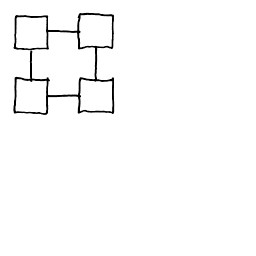
\includegraphics[width = 5cm]{../TikZ/drawings/expert-64.png}&
        \begin{minipage}{10cm}
        \begin{verbatim}
      reflect(x = 6)
      Line(1,2,1,4,arrow = False,solid = True)
            reflect(y = 6)
            Line(2,5,4,5,arrow = False,solid = True)
            Rectangle(0,0,2,2)
        \end{verbatim}
\end{minipage}
\end{tabular}        
        \\

        \begin{tabular}{ll}
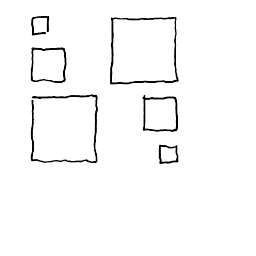
\includegraphics[width = 5cm]{../TikZ/drawings/expert-36.png}&
        \begin{minipage}{10cm}
        \begin{verbatim}
  for (2)
      Rectangle(5 * i + None,5 * i + None,5 * i + 4,5 * i + 4)
      Rectangle(7 * i + None,-3 * i + 5,7 * i + 2,-3 * i + 7)
      Rectangle(8 * i + None,-8 * i + 8,8 * i + 1,-8 * i + 9)
        \end{verbatim}
\end{minipage}
\end{tabular}        
        \\

        \begin{tabular}{ll}
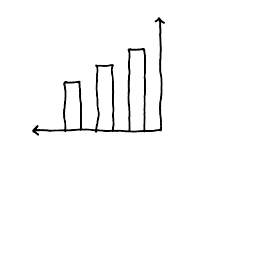
\includegraphics[width = 5cm]{../TikZ/drawings/expert-58.png}&
        \begin{minipage}{10cm}
        \begin{verbatim}
  for (3)
      Line(8,0,8 * i + -8,7 * i + -7,arrow = True,solid = True)
      Rectangle(2 * i + 2,0,2 * i + 3,None * i + 3)
        \end{verbatim}
\end{minipage}
\end{tabular}        
        \\

        \begin{tabular}{ll}
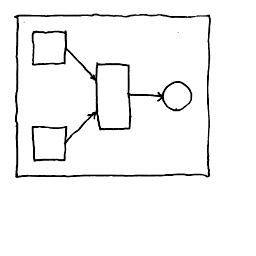
\includegraphics[width = 5cm]{../TikZ/drawings/expert-3.png}&
        \begin{minipage}{10cm}
        \begin{verbatim}
      reflect(y = 10)
      Circle(10,5)
        for (2)
            Line(-4 * i + 7,-3 * i + 5,-4 * i + 9,-1 * i + 5,arrow = True,solid = True)
            Rectangle(24 * i + 5,3,-18 * i + 7,7)
            Rectangle(-1 * i + 1,-1 * i + 1,9 * i + 3,7 * i + 3)
        \end{verbatim}
\end{minipage}
\end{tabular}        
        \\

        \begin{tabular}{ll}

\includegraphics[width = 5cm]{../TikZ/drawings/expert-28.png}&
        \begin{minipage}{10cm}
        \begin{verbatim}
  Line(0,2,2,2,arrow = False,solid = True)
  Line(0,0,0,2,arrow = False,solid = True)
  Line(0 * None + None,0,0,2,arrow = False,solid = True)
        \end{verbatim}
\end{minipage}
\end{tabular}        
        \\

        \begin{tabular}{ll}
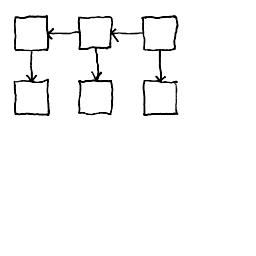
\includegraphics[width = 5cm]{../TikZ/drawings/expert-22.png}&
        \begin{minipage}{10cm}
        \begin{verbatim}
  for (3)
      Line(4 * i + 1,4,4 * i + 1,2,arrow = True,solid = True)
      Line(4 * i + None,5,4 * i + -2,5,arrow = True,solid = True)
      Rectangle(-4 * i + 8,4,-4 * i + 10,6)
      Rectangle(-4 * i + 8,0,-4 * i + 10,2)
        \end{verbatim}
\end{minipage}
\end{tabular}        
        \\

        \begin{tabular}{ll}
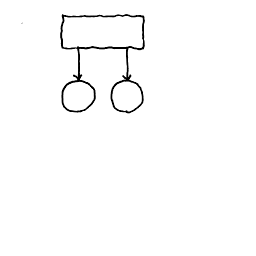
\includegraphics[width = 5cm]{../TikZ/drawings/expert-69.png}&
        \begin{minipage}{10cm}
        \begin{verbatim}
  Rectangle(0,4,5,6)
        reflect(x = 5)
        Circle(4,1)
        Line(1,4,1,2,arrow = True,solid = True)
        \end{verbatim}
\end{minipage}
\end{tabular}        
        \\

        \begin{tabular}{ll}
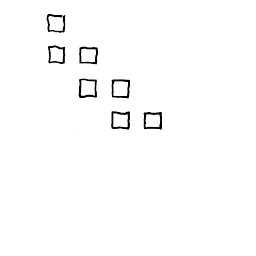
\includegraphics[width = 5cm]{../TikZ/drawings/expert-14.png}&
        \begin{minipage}{10cm}
        \begin{verbatim}
  for (4)
      Rectangle(-2 * i + 6,2 * i + -2,-2 * i + 7,2 * i + -1)
      Rectangle(2 * i + None,-2 * i + 6,2 * i + 1,-2 * i + 7)
        \end{verbatim}
\end{minipage}
\end{tabular}        
        \\

        \begin{tabular}{ll}
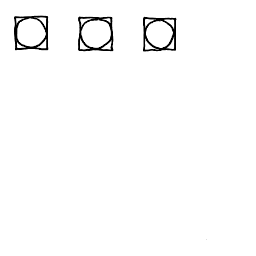
\includegraphics[width = 5cm]{../TikZ/drawings/expert-68.png}&
        \begin{minipage}{10cm}
        \begin{verbatim}
  for (4)
      Circle(-4 * i + 9,1)
      Rectangle(4 * i + -4,0,4 * i + -2,2)
        \end{verbatim}
\end{minipage}
\end{tabular}        
        \\

        \begin{tabular}{ll}
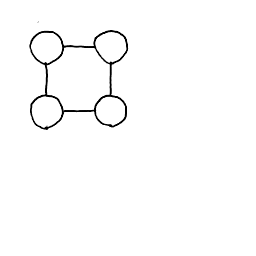
\includegraphics[width = 5cm]{../TikZ/drawings/expert-65.png}&
        \begin{minipage}{10cm}
        \begin{verbatim}
      reflect(x = 6)
      Line(1,2,1,4,arrow = False,solid = True)
            reflect(y = 6)
            Circle(5,5)
            Line(2,5,4,5,arrow = False,solid = True)
        \end{verbatim}
\end{minipage}
\end{tabular}        
        \\

        \begin{tabular}{ll}
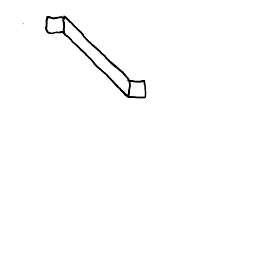
\includegraphics[width = 5cm]{../TikZ/drawings/expert-67.png}&
        \begin{minipage}{10cm}
        \begin{verbatim}
  Line(1,5,5,1,arrow = False,solid = True)
  Line(1,4,5,0,arrow = False,solid = True)
  Rectangle(0,4,1,5)
  Rectangle(5,0,6,1)
  Line(1 * None + None,4,5,0,arrow = False,solid = True)
        \end{verbatim}
\end{minipage}
\end{tabular}        
        \\

        \begin{tabular}{ll}
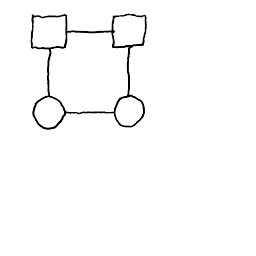
\includegraphics[width = 5cm]{../TikZ/drawings/expert-12.png}&
        \begin{minipage}{10cm}
        \begin{verbatim}
  Line(2,1,5,1,arrow = False,solid = True)
        reflect(x = 7)
        Circle(1,1)
        Line(1,2,1,5,arrow = False,solid = True)
        Line(2,6,5,6,arrow = False,solid = True)
        Rectangle(5,5,7,7)
        \end{verbatim}
\end{minipage}
\end{tabular}        
        \\

        \begin{tabular}{ll}
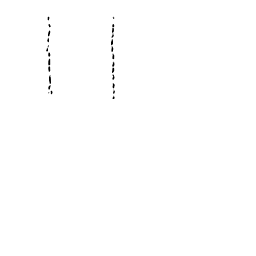
\includegraphics[width = 5cm]{../TikZ/drawings/expert-42.png}&
        \begin{minipage}{10cm}
        \begin{verbatim}
  Line(0,0,0,5,arrow = False,solid = False)
  Line(4,1,4,5,arrow = False,solid = False)
  Line(4,0,4,1,arrow = False,solid = False)
  Line(0 * None + None,0,4,1,arrow = False,solid = False)
        \end{verbatim}
\end{minipage}
\end{tabular}        
        \\

        \begin{tabular}{ll}

\includegraphics[width = 5cm]{../TikZ/drawings/expert-10.png}&
        \begin{minipage}{10cm}
        \begin{verbatim}
  Rectangle(0,0,3,4)
        \end{verbatim}
\end{minipage}
\end{tabular}        
        \\

        \begin{tabular}{ll}
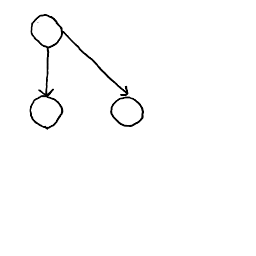
\includegraphics[width = 5cm]{../TikZ/drawings/expert-35.png}&
        \begin{minipage}{10cm}
        \begin{verbatim}
  Circle(6,1)
    for (2)
        Circle(1,5 * i + 1)
        Line(None * i + 1,None * i + 5,5 * i + 1,2,arrow = True,solid = True)
        \end{verbatim}
\end{minipage}
\end{tabular}        
        \\

        \begin{tabular}{ll}
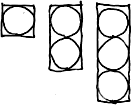
\includegraphics[width = 5cm]{../TikZ/drawings/expert-31.png}&
        \begin{minipage}{10cm}
        \begin{verbatim}
  Circle(4,5)
    for (4)
        Circle(-3 * i + 10,2 * i + -1)
        Circle(7,2 * i + -1)
        Rectangle(-3 * i + 9,2 * i + -2,-3 * i + 11,6)
        \end{verbatim}
\end{minipage}
\end{tabular}        
        \\

        \begin{tabular}{ll}
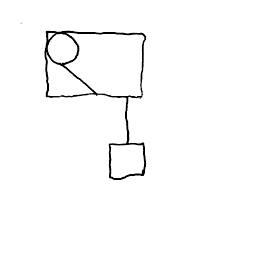
\includegraphics[width = 5cm]{../TikZ/drawings/expert-37.png}&
        \begin{minipage}{10cm}
        \begin{verbatim}
  Circle(1,8)
    for (4)
        Line(4 * i + 1,-5 * i + 7,2 * i + 3,5,arrow = False,solid = True)
        Rectangle(4 * i + -8,-5 * i + 15,6,-7 * i + 23)
        \end{verbatim}
\end{minipage}
\end{tabular}        
        \\

        \begin{tabular}{ll}
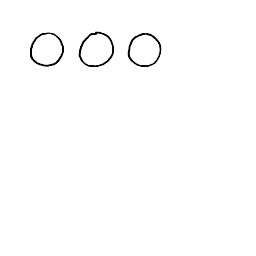
\includegraphics[width = 5cm]{../TikZ/drawings/expert-40.png}&
        \begin{minipage}{10cm}
        \begin{verbatim}
  Circle(1,1)
        reflect(x = 11)
        Circle(4,1)
        \end{verbatim}
\end{minipage}
\end{tabular}        
        \\

        \begin{tabular}{ll}

\includegraphics[width = 5cm]{../TikZ/drawings/expert-29.png}&
        \begin{minipage}{10cm}
        \begin{verbatim}
  for (3)
      Line(None * i + None,-1 * i + 6,4 * i + -2,-1 * i + 6,arrow = False,solid = True)
      Line(None * i + None,-2 * i + 4,None * i + None,-1 * i + 6,arrow = False,solid = True)
      Line(-2 * i + 2,None * i + 5,-2 * i + 4,None * i + 5,arrow = False,solid = True)
        \end{verbatim}
\end{minipage}
\end{tabular}        
        \\

        \begin{tabular}{ll}
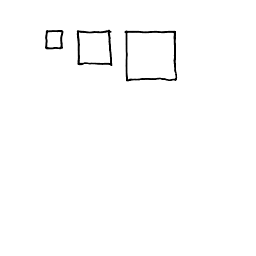
\includegraphics[width = 5cm]{../TikZ/drawings/expert-62.png}&
        \begin{minipage}{10cm}
        \begin{verbatim}
  Rectangle(5,0,8,3)
  Rectangle(2,1,4,3)
  Rectangle(0,2,1,3)
  Rectangle(2 * None + None,0,8,3)
        \end{verbatim}
\end{minipage}
\end{tabular}        
        \\

        \begin{tabular}{ll}
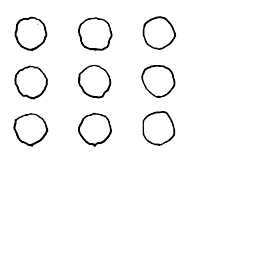
\includegraphics[width = 5cm]{../TikZ/drawings/expert-57.png}&
        \begin{minipage}{10cm}
        \begin{verbatim}
  for (3)
      Circle(-4 * i + 9,4)
      Circle(-4 * i + 9,1)
      Circle(4 * i + 1,7)
        \end{verbatim}
\end{minipage}
\end{tabular}        
        \\

        \begin{tabular}{ll}
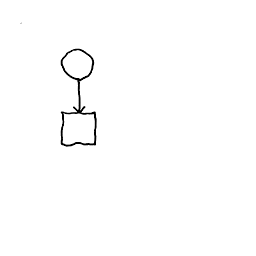
\includegraphics[width = 5cm]{../TikZ/drawings/expert-55.png}&
        \begin{minipage}{10cm}
        \begin{verbatim}
  Circle(1,5)
  Line(1,4,1,2,arrow = True,solid = True)
  Rectangle(0,0,2,2)
  Circle(1,None * None + None)
        \end{verbatim}
\end{minipage}
\end{tabular}        
        \\

        \begin{tabular}{ll}

\includegraphics[width = 5cm]{../TikZ/drawings/expert-66.png}&
        \begin{minipage}{10cm}
        \begin{verbatim}
  Line(1,1,6,1,arrow = False,solid = True)
  Line(0,2,7,2,arrow = False,solid = True)
  Line(2,0,5,0,arrow = False,solid = True)
  Line(2 * None + None,1,6,1,arrow = False,solid = True)
        \end{verbatim}
\end{minipage}
\end{tabular}        
        \\

        \begin{tabular}{ll}
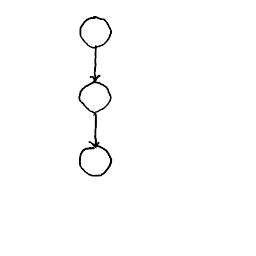
\includegraphics[width = 5cm]{../TikZ/drawings/expert-26.png}&
        \begin{minipage}{10cm}
        \begin{verbatim}
  Line(1,3,1,4,arrow = False,solid = True)
    for (3)
        Circle(1,-4 * i + 9)
        Line(1,-5 * i + 8,1,-4 * i + 6,arrow = True,solid = True)
        \end{verbatim}
\end{minipage}
\end{tabular}        
        \\

        \begin{tabular}{ll}

\includegraphics[width = 5cm]{../TikZ/drawings/expert-15.png}&
        \begin{minipage}{10cm}
        \begin{verbatim}
  Line(1,2,3,2,arrow = False,solid = True)
  Line(0,3,2,3,arrow = False,solid = False)
  Line(3,0,5,0,arrow = False,solid = True)
  Line(2,1,4,1,arrow = False,solid = False)
  Line(1 * None + None,1,4,1,arrow = False,solid = False)
        \end{verbatim}
\end{minipage}
\end{tabular}        
        \\

        \begin{tabular}{ll}
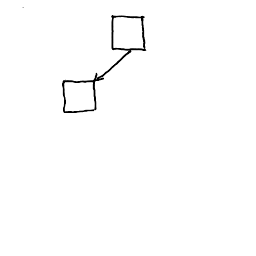
\includegraphics[width = 5cm]{../TikZ/drawings/expert-19.png}&
        \begin{minipage}{10cm}
        \begin{verbatim}
  Line(4,4,2,2,arrow = True,solid = True)
  Rectangle(3,4,5,6)
  Rectangle(0,0,2,2)
  Line(4,4,2,2,arrow = True,solid = True)
        \end{verbatim}
\end{minipage}
\end{tabular}        
        \\

        \begin{tabular}{ll}

\includegraphics[width = 5cm]{../TikZ/drawings/expert-8.png}&
        \begin{minipage}{10cm}
        \begin{verbatim}
  Line(0,0,0,4,arrow = False,solid = True)
  Line(0,0,0,4,arrow = False,solid = True)
        \end{verbatim}
\end{minipage}
\end{tabular}        
        \\

        \begin{tabular}{ll}
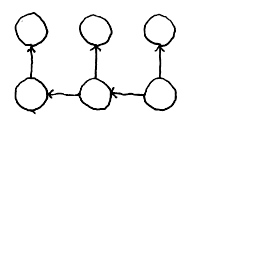
\includegraphics[width = 5cm]{../TikZ/drawings/expert-23.png}&
        \begin{minipage}{10cm}
        \begin{verbatim}
  Line(4,1,2,1,arrow = False,solid = True)
    for (3)
        Circle(-4 * i + 9,5)
        Circle(-4 * i + 9,1)
        Line(-1 * i + 9,-1 * i + 2,-3 * i + 9,-3 * i + 4,arrow = True,solid = False)
        Line(-4 * i + 5,2,-4 * i + 5,4,arrow = True,solid = True)
        \end{verbatim}
\end{minipage}
\end{tabular}        
        \\

        \begin{tabular}{ll}
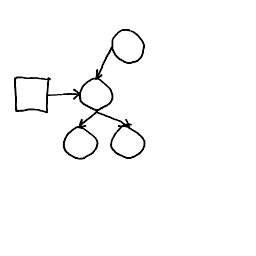
\includegraphics[width = 5cm]{../TikZ/drawings/expert-60.png}&
        \begin{minipage}{10cm}
        \begin{verbatim}
  Rectangle(0,3,2,5)
    for (2)
        Circle(3 * i + 4,1)
        Circle(2 * i + 5,3 * i + 4)
        Line(-1 * i + 6,-4 * i + 7,-1 * i + 5,-3 * i + 5,arrow = True,solid = True)
        Line(-3 * i + 5,None * i + 3,-3 * i + 7,2 * i + 2,arrow = True,solid = True)
        \end{verbatim}
\end{minipage}
\end{tabular}        
        \\

        \begin{tabular}{ll}
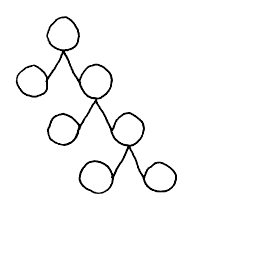
\includegraphics[width = 5cm]{../TikZ/drawings/expert-16.png}&
        \begin{minipage}{10cm}
        \begin{verbatim}
  for (4)
      Circle(2 * i + 3,-3 * i + 10)
      Circle(2 * i + 1,-3 * i + 7)
      Line(2 * i + 3,-3 * i + 9,2 * i + 4,-3 * i + 7,arrow = False,solid = True)
      Line(-2 * i + 8,3 * i + -2,-2 * i + 9,3 * i + None,arrow = False,solid = True)
        \end{verbatim}
\end{minipage}
\end{tabular}        
        \\

        \begin{tabular}{ll}
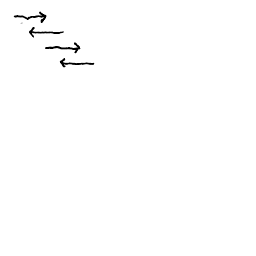
\includegraphics[width = 5cm]{../TikZ/drawings/expert-13.png}&
        \begin{minipage}{10cm}
        \begin{verbatim}
  Line(5,0,3,0,arrow = True,solid = True)
  Line(2,1,4,1,arrow = True,solid = True)
  Line(0,3,2,3,arrow = True,solid = True)
  Line(3,2,1,2,arrow = True,solid = True)
  Line(2 * None + None,2,1,2,arrow = True,solid = True)
        \end{verbatim}
\end{minipage}
\end{tabular}        
        \\

        \begin{tabular}{ll}
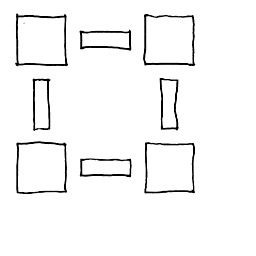
\includegraphics[width = 5cm]{../TikZ/drawings/expert-47.png}&
        \begin{minipage}{10cm}
        \begin{verbatim}
      reflect(x = 11)
      Rectangle(9,4,10,7)
            reflect(y = 11)
            Rectangle(0,0,3,3)
            Rectangle(4,9,7,10)
        \end{verbatim}
\end{minipage}
\end{tabular}        
        \\

        \begin{tabular}{ll}
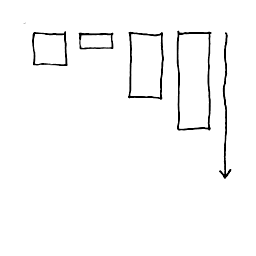
\includegraphics[width = 5cm]{../TikZ/drawings/expert-5.png}&
        \begin{minipage}{10cm}
        \begin{verbatim}
  Line(12,9,12,0,arrow = True,solid = True)
    for (2)
        Rectangle(-3 * i + 9,2 * i + 3,-3 * i + 11,9)
        Rectangle(3 * i + None,None * i + 7,3 * i + 2,9)
        \end{verbatim}
\end{minipage}
\end{tabular}        
        \\

        \begin{tabular}{ll}

\includegraphics[width = 5cm]{../TikZ/drawings/expert-59.png}&
        \begin{minipage}{10cm}
        \begin{verbatim}
  Line(4,0,0,0,arrow = False,solid = False)
  Line(4,0,0,0,arrow = False,solid = False)
        \end{verbatim}
\end{minipage}
\end{tabular}        
        \\

        \begin{tabular}{ll}
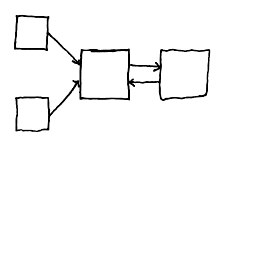
\includegraphics[width = 5cm]{../TikZ/drawings/expert-50.png}&
        \begin{minipage}{10cm}
        \begin{verbatim}
  Line(8,3,9,3,arrow = False,solid = True)
    for (2)
        Line(-6 * i + 8,3 * i + 3,-3 * i + 7,None * i + 3,arrow = True,solid = True)
        Line(5 * i + 2,3 * i + 1,5 * i + 4,None * i + 3,arrow = True,solid = True)
        Rectangle(9 * i + None,2 * i + None,10 * i + 2,3 * i + 2)
        Rectangle(4 * i + None,-3 * i + 5,5 * i + 2,-2 * i + 7)
        \end{verbatim}
\end{minipage}
\end{tabular}        
        \\

        \begin{tabular}{ll}
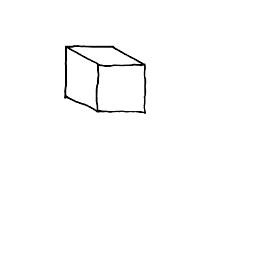
\includegraphics[width = 5cm]{../TikZ/drawings/expert-6.png}&
        \begin{minipage}{10cm}
        \begin{verbatim}
  Line(0,4,3,4,arrow = False,solid = True)
    for (2)
        Line(3 * i + None,3 * i + 1,3 * i + 2,3 * i + None,arrow = False,solid = True)
        Line(0,3 * i + 1,2 * i + None,-1 * i + 4,arrow = False,solid = True)
        Rectangle(2,-8 * i + 8,29 * i + -24,12 * i + -9)
        \end{verbatim}
\end{minipage}
\end{tabular}        
        